\chapter{Coordinates}

%-----------------------------------------------------------------------------
\section{Reference Orbit}
\label{s:ref}

The ``reference orbit'' is the path of a ``reference particle'' and is
used to define a coordinate system for actual particles (whose orbits
are simulated in \bmad) as shown in Figure~\ref{f:local_coords}. At a
given time $t$ the reference particle is a distance $s = c \, t$ along
the reference orbit from the zero position of the reference orbit. The
origin of the local $(x, y, z)$ coordinate system at time $t$ is at the
reference particle with the $z$--axis tangent to the reference
orbit and pointing in the direction of the reference particle
motion. The $x$ and $y$--axes are perpendicular to the reference
orbit. If there are no vertical bends, the $y$--axis is in the
vertical direction and the $x$--axis is in the horizontal plane.

\begin{figure}[tb]
\centering
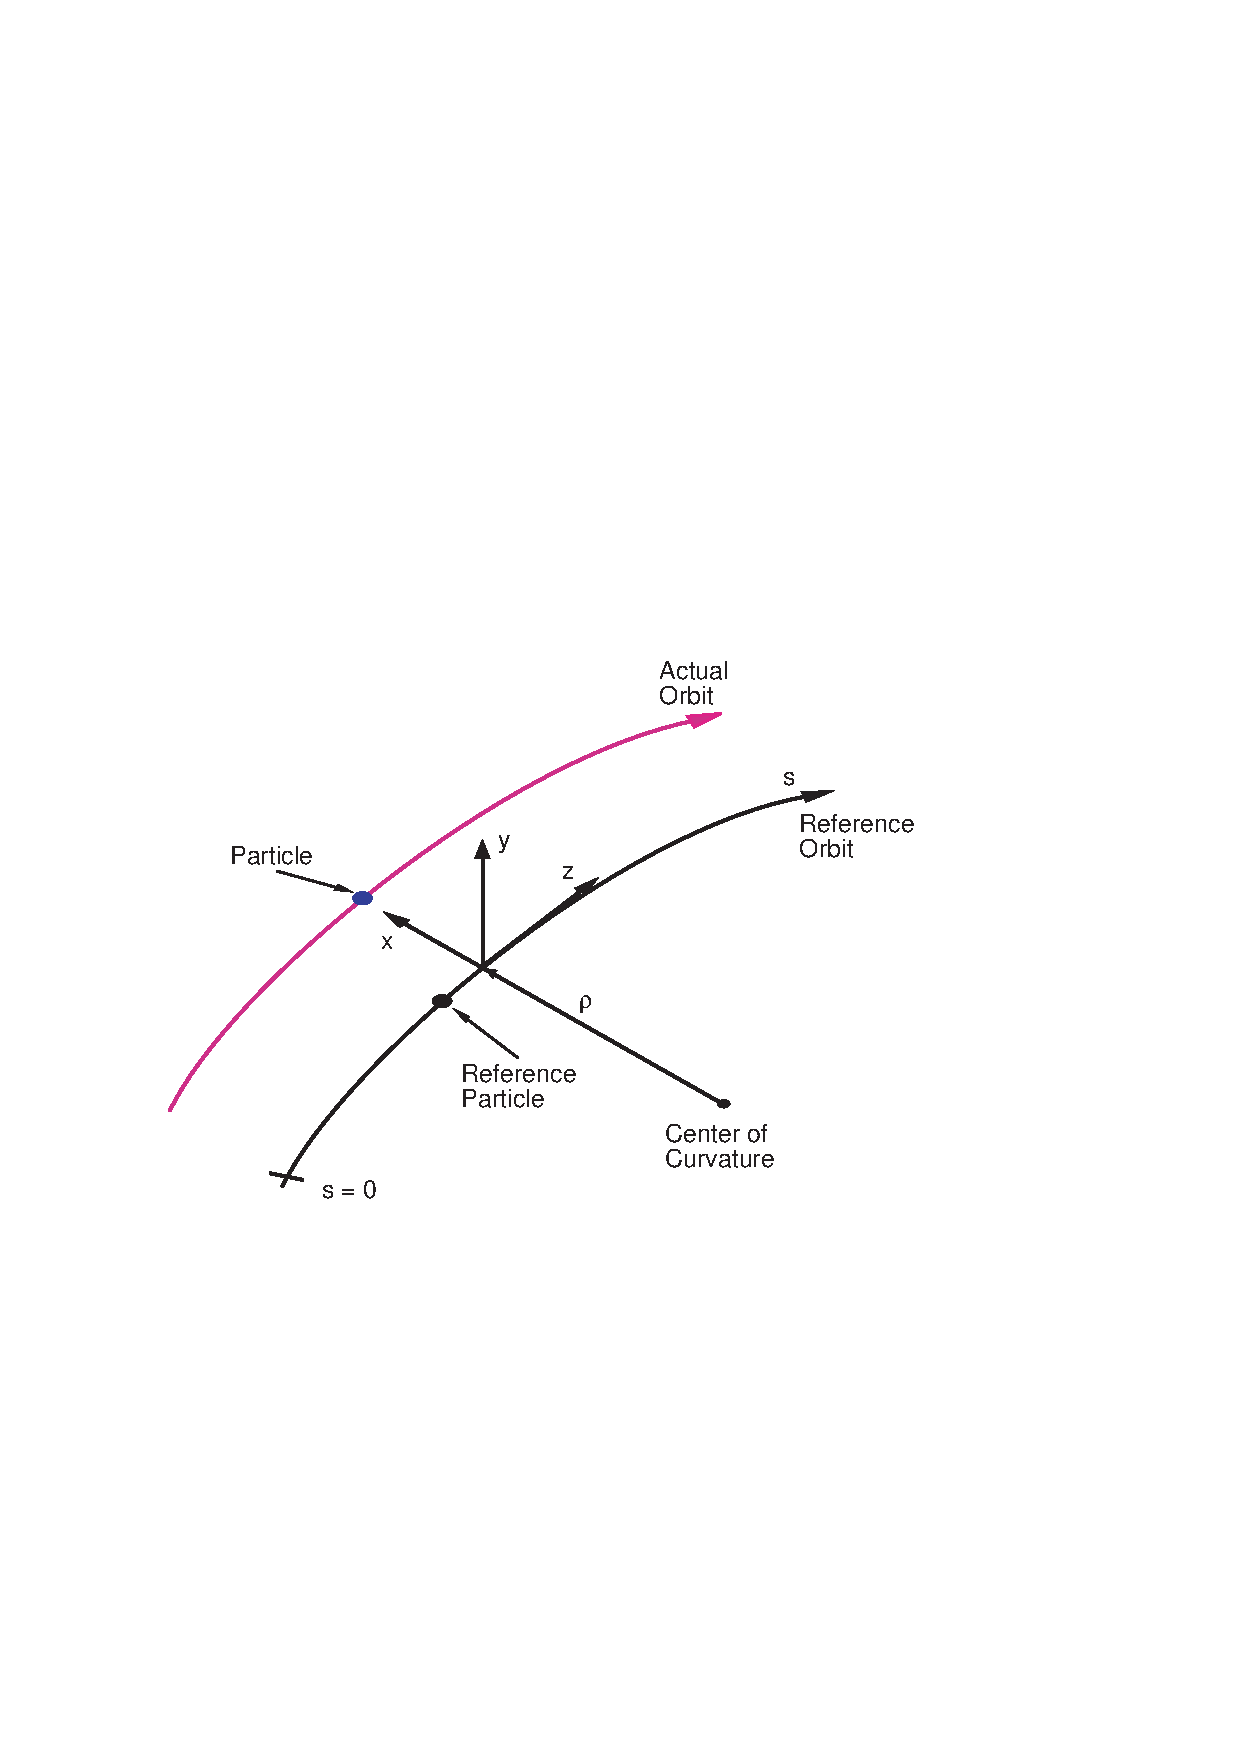
\includegraphics{local_coords.psfig}
\caption{The Local Reference System}
\label{f:local_coords}
\end{figure}

In \bmad, a lattice is comprised of a sequence of elements such as
quadrupoles, bends, rfcavities, etc. Each element has an entrance
point, an exit point, and a reference curve between them. For a bend,
the reference curve is a segment of a circular arc. For all other
elements, the reference curve is a straight line segment.  The
reference orbit is constructed by arranging the elements so that the
exit point of one element coincides with the entrance point of the
next with the reference curves forming an arc with no kinks.
The reference orbit is then the sum of the reference curves. If
not specified otherwise, the $s = 0$ position is the entrance
point of the first element.

Notice that, in a wiggler, the reference orbit, which is a straight
line, does {\em not} correspond to the orbit that any actual particle
could travel. Typically the physical entity of an element is centered
about the reference curve, However, by specifying offsets and pitches
(See Section~\ref{s:offset}), the center line of an element may be
arbitrarily oriented with respect to its reference curve. Since the
reference curve of an element is fixed to the reference curves of the
neighboring elements, setting a nonzero offset or pitch
for an element moves the physical magnet and does not affect the
reference curve. Shifting a physical magnet with respect to its
reference curve generally means that the reference curve does {\em
not} correspond to the orbit that any actual particle could travel.

%-----------------------------------------------------------------------------
\section{Global Reference System}
\label{s:global}

The global reference system describes the orientation of the reference
orbit with respect to the laboratory coordinate system.  \bmad,
following the \mad\ convention, uses a Cartesian coordinate system
$(X, Y, Z)$ for the global reference system, along with three angles
$\theta, \phi, \psi$ used to define the reference orbit's orientation
as shown in Figure~\ref{f:global_coords}. Conventionally $Y$ is the
vertical coordinate and $(X, Z)$ are the ``floor'' coordinates.  The
three angles are defined as follows:
\begin{description}
\item[$\theta$ Azimuth angle:] Angle in the $(X, Z)$ plane 
between the $Z$--axis and the projection of the $z$--axis onto the
$(X, Z)$ plane. A positive angle of $\theta = \pi/2$ corresponds to the
projected $z$--axis pointing in the positive $X$ direction.
\item[$\phi$ Pitch (elevation) angle:] Angle between the $z$--axis 
and the $Y$--axis. A positive angle of $\phi = \pi/2$ corresponds to
the $s$--axis pointing in the positive $Y$ direction.
\item[$\psi$ Roll angle:] Angle of the $x$--axis with respect 
to the intersection of the $(X, Z)$ plane with the $(x, y)$ plane. A
positive $\psi$ forms a right--handed screw with the $s$--axis.
\end{description}

\begin{figure}
\centering
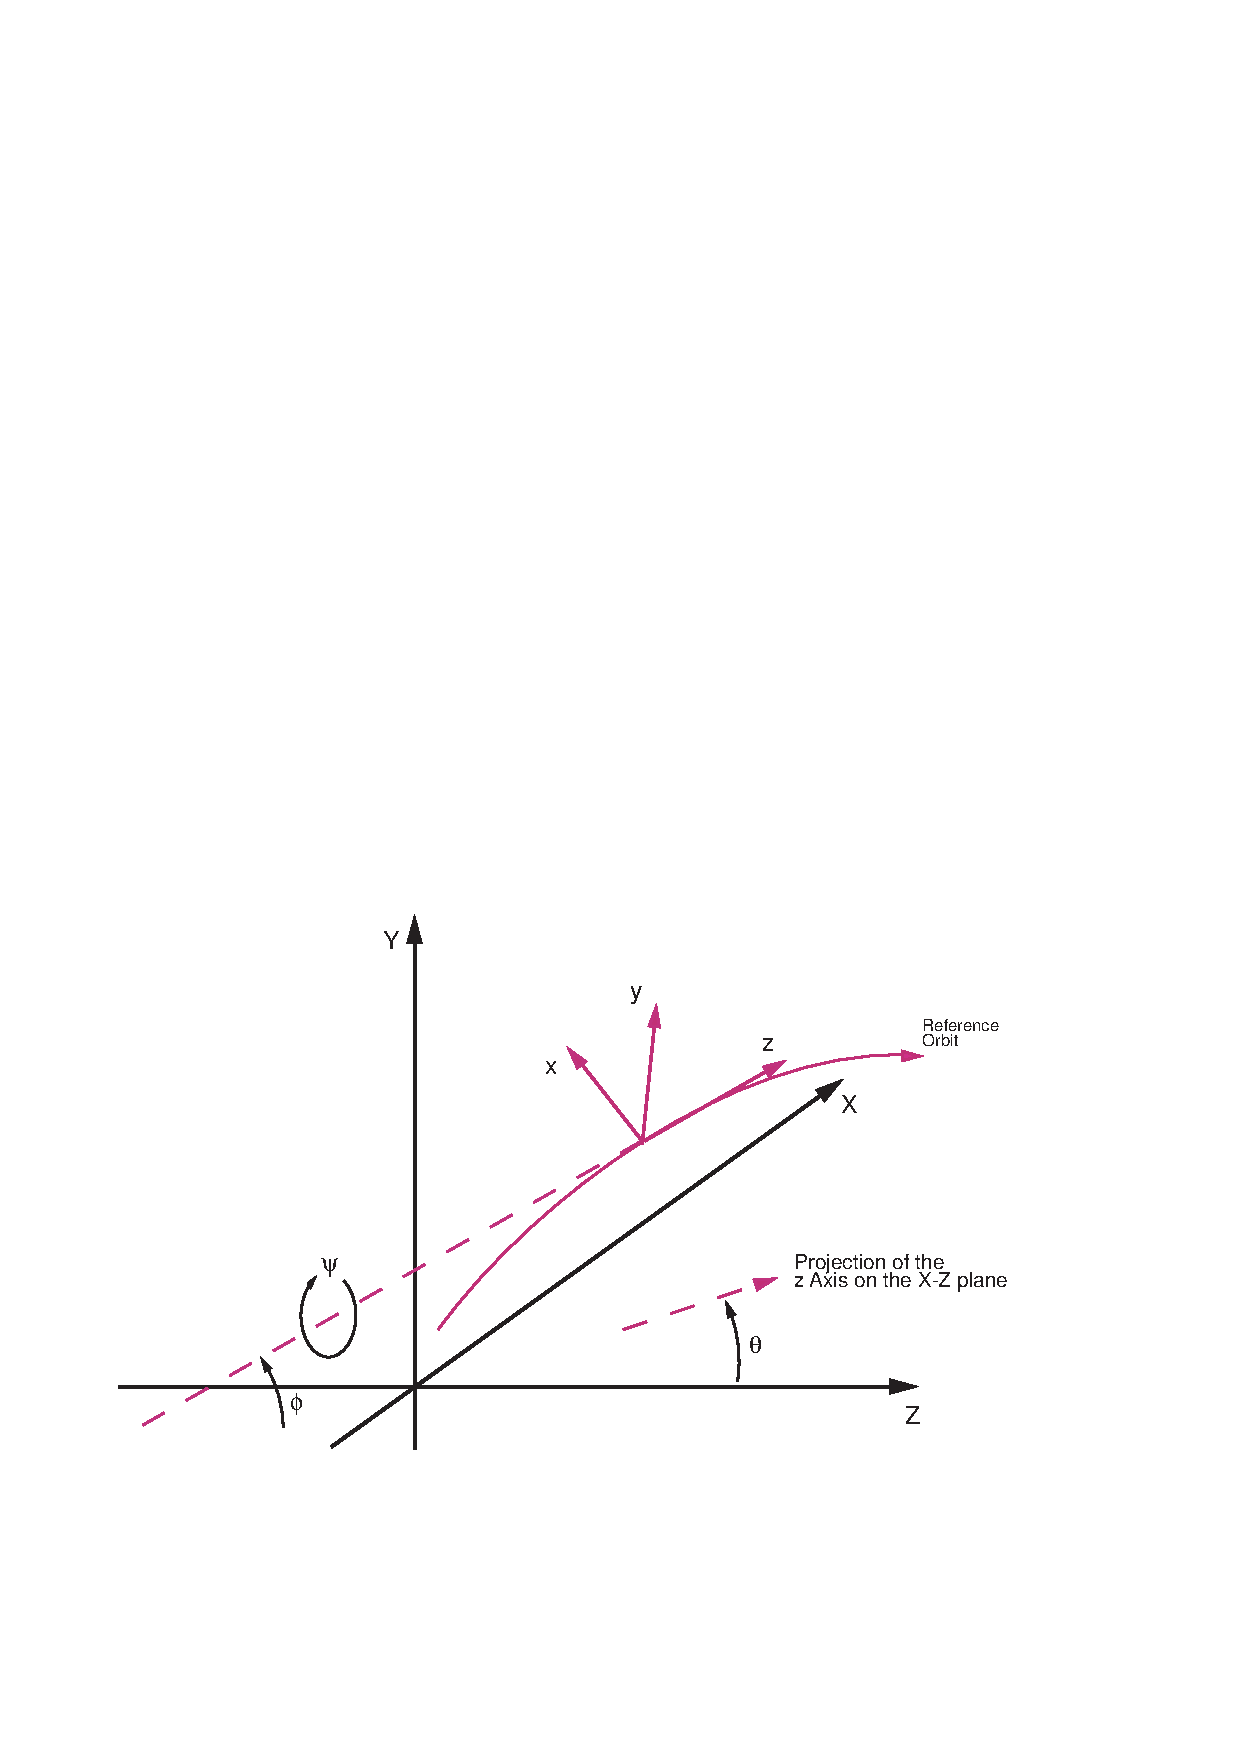
\includegraphics{global_coords.psfig}
\caption{The Global Reference System}
\label{f:global_coords}
\end{figure}

By default, the reference orbit's origin coincides with the
$(X, Y, Z)$ origin and at $s = 0$ the $x$, $y$, and $z$ axes
correspond to the $X$, $Y$, and $Z$ axes respectively. $\theta$
decreases as one follows the reference orbit when going through a
horizontal bend with a positive bending angle. This corresponds to $x$
pointing radially outward. Without any vertical bends, the $Y$ and $y$
axes will coincide, and $\phi$ and $\psi$ will both be zero.

\vfill

%-----------------------------------------------------------------------------
\section{Phase Space Coordinate System}

\bmad uses the canonical phase space coordinates 
$(x, p_x, y, p_y, z, p_z)$. $x$, $y$, and $z$ are the
coordinates with respect to the reference particle as explained in
Section~\ref{s:ref}. $p_x$ and $p_y$ are the normalized momenta
\begin{align}
  p_x = &\frac{P_x}{P_0} \\
  p_y = &\frac{P_y}{P_0}
\end{align}
where $P_x$ and $P_y$ are, respectively, the momentum components along the $x$ and
$y$ axes, and $P_0$ is the reference (sometimes called the
design) momentum. The longitudinal canonical momentum $p_z$ is given by
\begin{equation}
  p_z = \frac{\Delta E}{E_0}
\end{equation}
where $E_0$ is the reference energy and $\Delta E = E - E_0$ is the
deviation of the particle's energy from the reference energy. \mad\ uses
a slightly different coordinate system where $(z, p_z)$ is
replaced by $(-c\Delta t, p_t)$. $\Delta t$ is the time
difference for a particle to pass a point relative to the reference
particle and $p_t \equiv \Delta E / P_0 c$. For highly relativistic
particles the two coordinate systems are identical. For
non-relativistic particles, \bmad\ is not to be trusted in any
case. \bmad\ generally uses the small angle (paraxial) approximation
where it is assumed that $p_x, p_y \ll 1$. With this approximation the
relationship between the canonical momenta and the slopes $x' \equiv dx/ds$
and $y' \equiv dy/ds$ is
\begin{align}
  x' &\approx \frac{p_x}{1 + p_z} (1 + g x) \\
  y' &\approx \frac{p_y}{1 + p_z} (1 + g x) 
\end{align}
where $g = 1/\rho$ is the curvature function with $\rho$ being the radius
of curvature of the reference orbit. $g = 0$ in a straight section.

For those programmers using the PTC software package directly (ignore
this if you don't know what I'm talking about) \'Etienne Forest uses a still
different coordinate system. where  $(z, p_z)$ is replaced by
$(\Delta E/P_0 c, c \Delta t)$